
\section{Cold Spray}\label{sec:cold-spray}
Most engineering alloys, including stainless steel, aluminium and titanium, will undergo solid-state bonding when two atomically flat and clean surfaces are brought into contact, particularly in vacuum environments where surface contamination is minimal~\cite{merstallinger2009coldwelding}. 
This phenomenon is known as cold welding and occurs because the surface energy of the separated metal interfaces is higher than that of the bonded state, making direct bonding thermodynamically favourable~\cite{WagleBaker2015}. 

In space applications, designs typically aim to prevent this but it is the core mechanism that underpins CSAM.\@ By accelerating metal powder particles to supersonic velocities and then impacting them upon the substrate, the particles cold weld to the surface forming a deposit. Seen in \autoref{fig:cs}, as the particles impact the surface they plastically deform, causing the disruption and removal of oxide layers and exposing unoxidised metal surfaces that bond upon contact. 
\begin{figure}[htbp]
    \centering
    
    \begin{minipage}{0.45\textwidth}
        \centering
        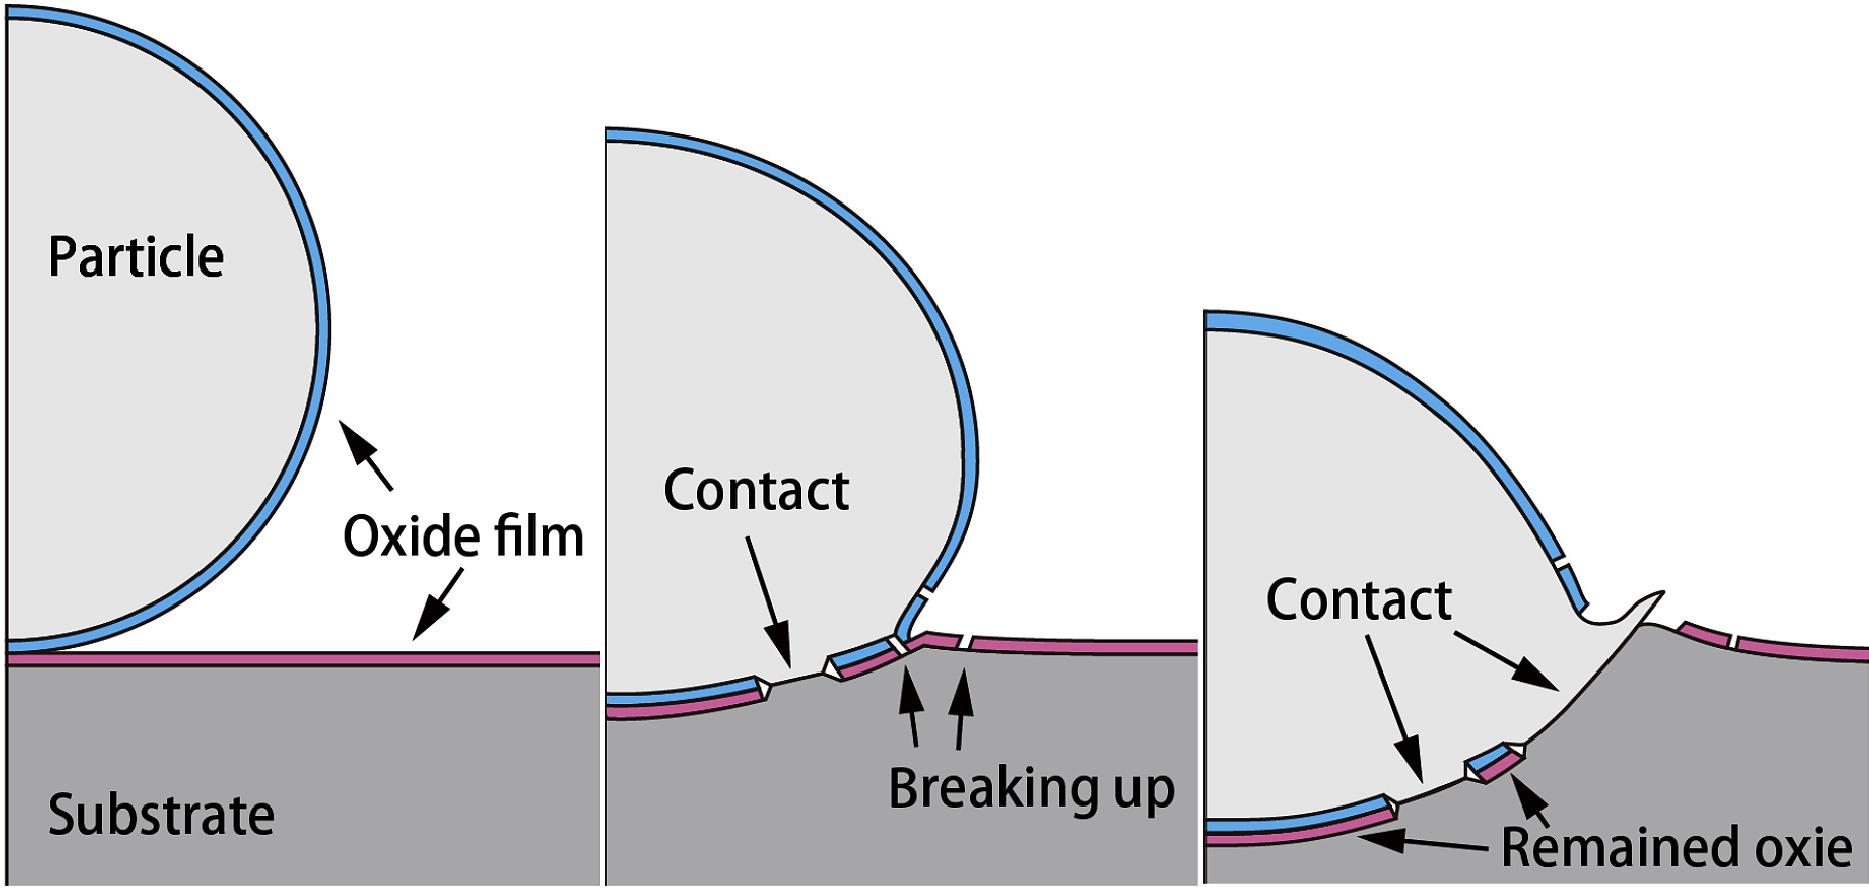
\includegraphics[width=\textwidth]{../report_assets/cs_bonding.png}
        \caption*{Deformation and Bonding on Impact~\cite{ZHANG2024137157}.}
    \end{minipage}
    \hfill
    \begin{minipage}{0.45\textwidth}
        \centering
        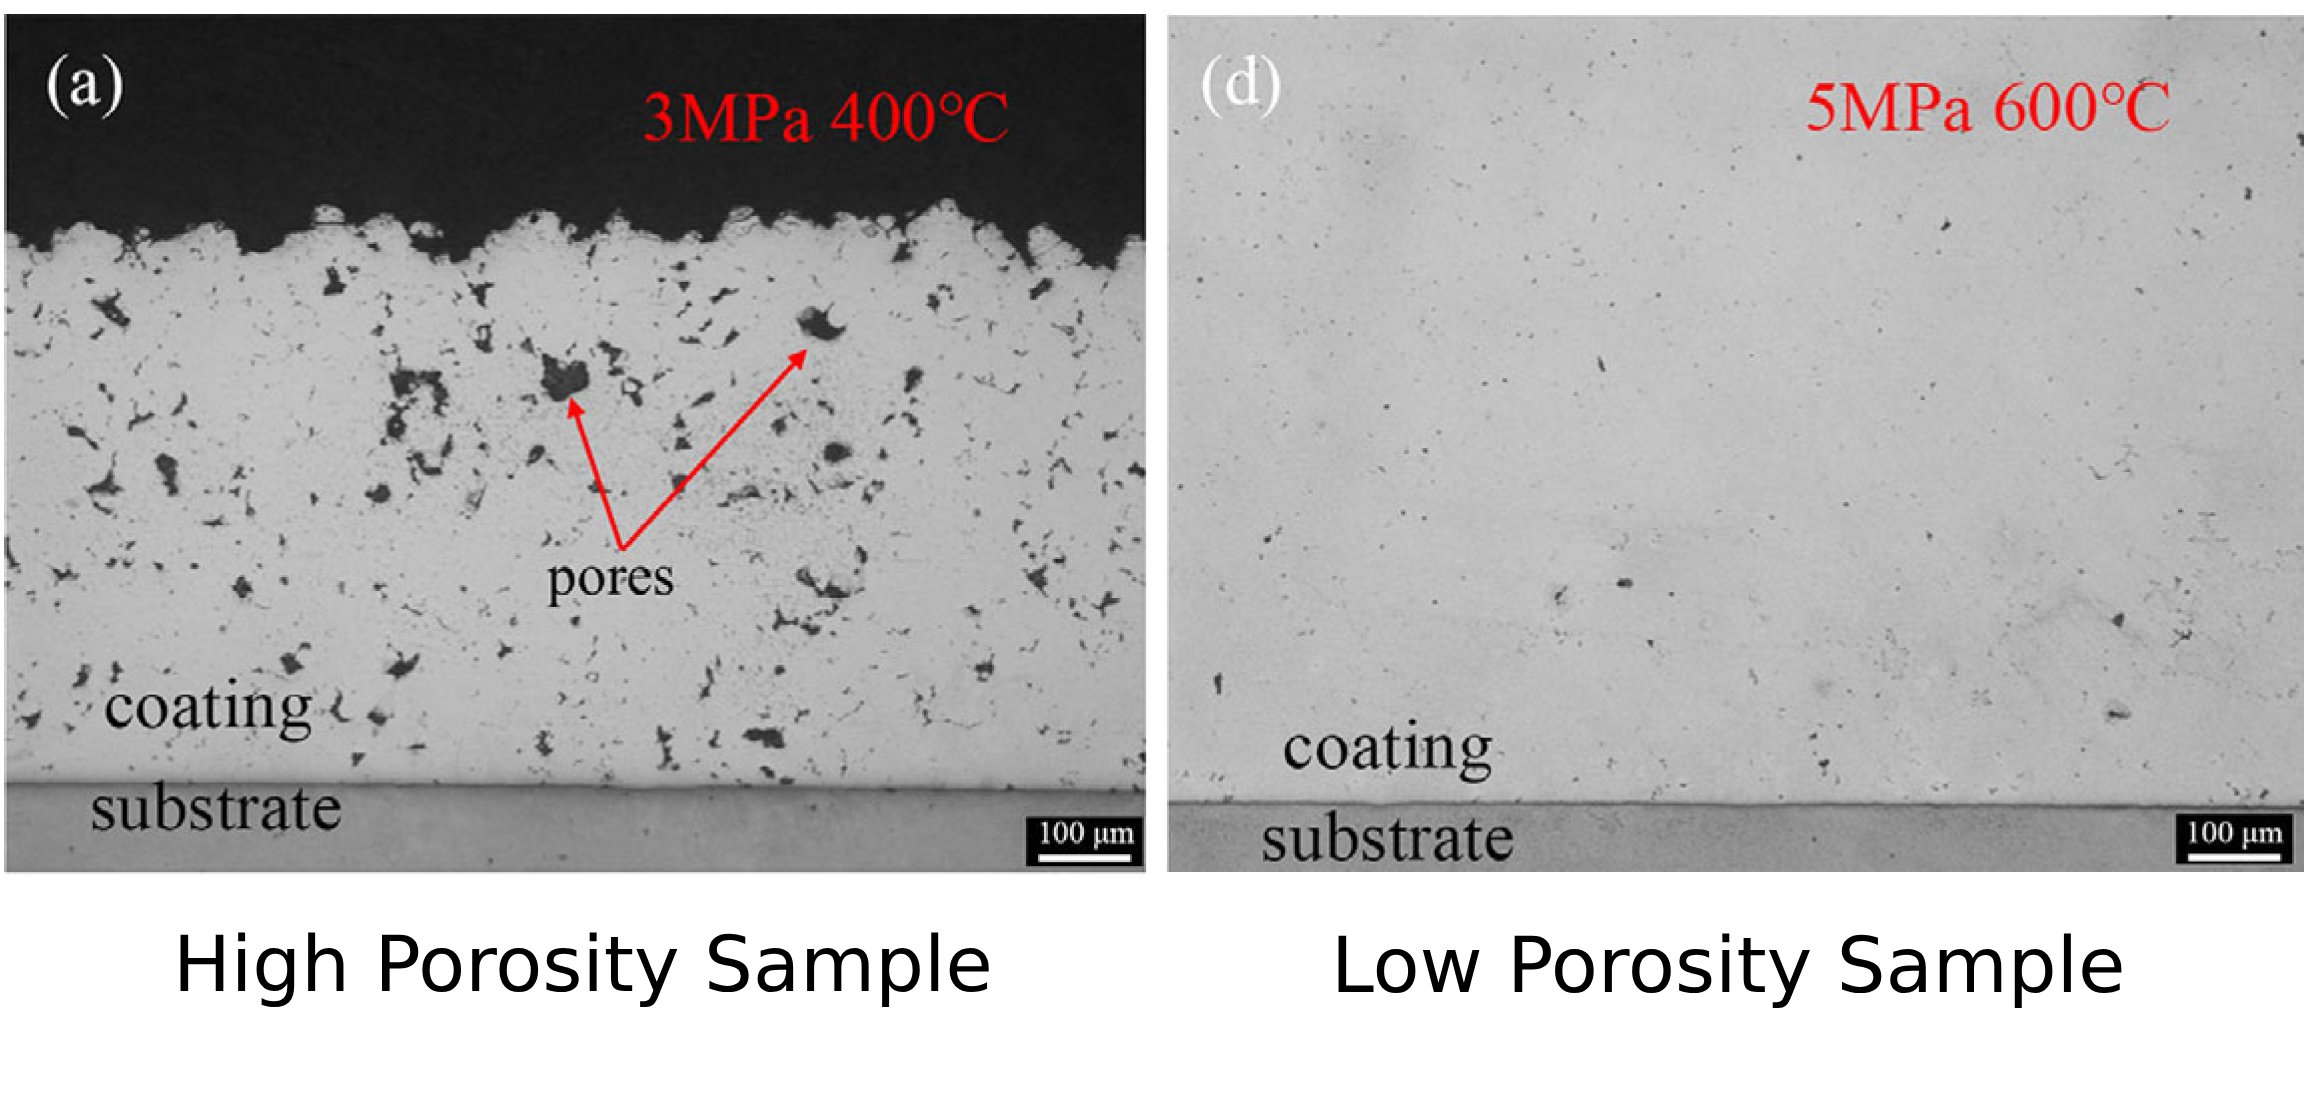
\includegraphics[width=\textwidth]{../report_assets/cs_porosity.png}
        \caption*{Do i need this one?~\cite{coatings13040738}.}
    \end{minipage}
    
\end{figure}\label{fig:cs}
The removal of oxide layers is thought to be because of adiabatic shear instability at the particle-substrate interface, which disrupts the brittle oxide shell and enables metallurgical bonding~\cite{assadi2016cold}. However, the precise mechanisms remain a topic of ongoing research and debate within the field~\cite{HASSANIGANGARAJ2018430}.

CSAM is a solid-state manufacturing process that builds material layers without ever melting the feedstock. Because the material never transitions through a liquid phase, thermal input remains low, preserving the original microstructure of both the powder and the underlying substrate, minimizing residual stresses and avoiding common fusion-related defects like porosity or solidification cracks. 

Arguably the most important parameters in the CSAM process is the velocity of the particle impacting the surface. If this velocity is too low then bonding does not occur and if it is too high the powder roughens or erodes the substrate. This velocity is dependent on the choice, pressure and temperature of accelerant gas and properties of the powder like mass flow rate, size, shape and hardness. 

An overview of cold spray coating in additive
manufacturing, component repairing and other
engineering applications could be useful paper to review for either images or citations/explanations
\newpage
\section{Fluidised Powder Bed Phenomenon}
Given that fluidisation underlies the design architecture presented later, the physics behind a generic fluidised powder-bed system are outlined in this section.
Fluidised powder beds exhibit distinctive fluid-mechanical behavior once a sufficient gas flow is passed upward through a granular solid~\cite{KuniiLevenspiel1977}. As the gas velocity increases from zero, the powder initially remains fixed with the gas passing through void spaces, known as a packed bed regime. At a critical threshold, the minimum fluidisation velocity, the drag force exerted by the gas equals the effective weight of the particles, causing the bed to loosen and particles to become suspended.
\begin{figure}[htbp]
    \centering
    
    \begin{minipage}{0.45\textwidth}
        \centering
        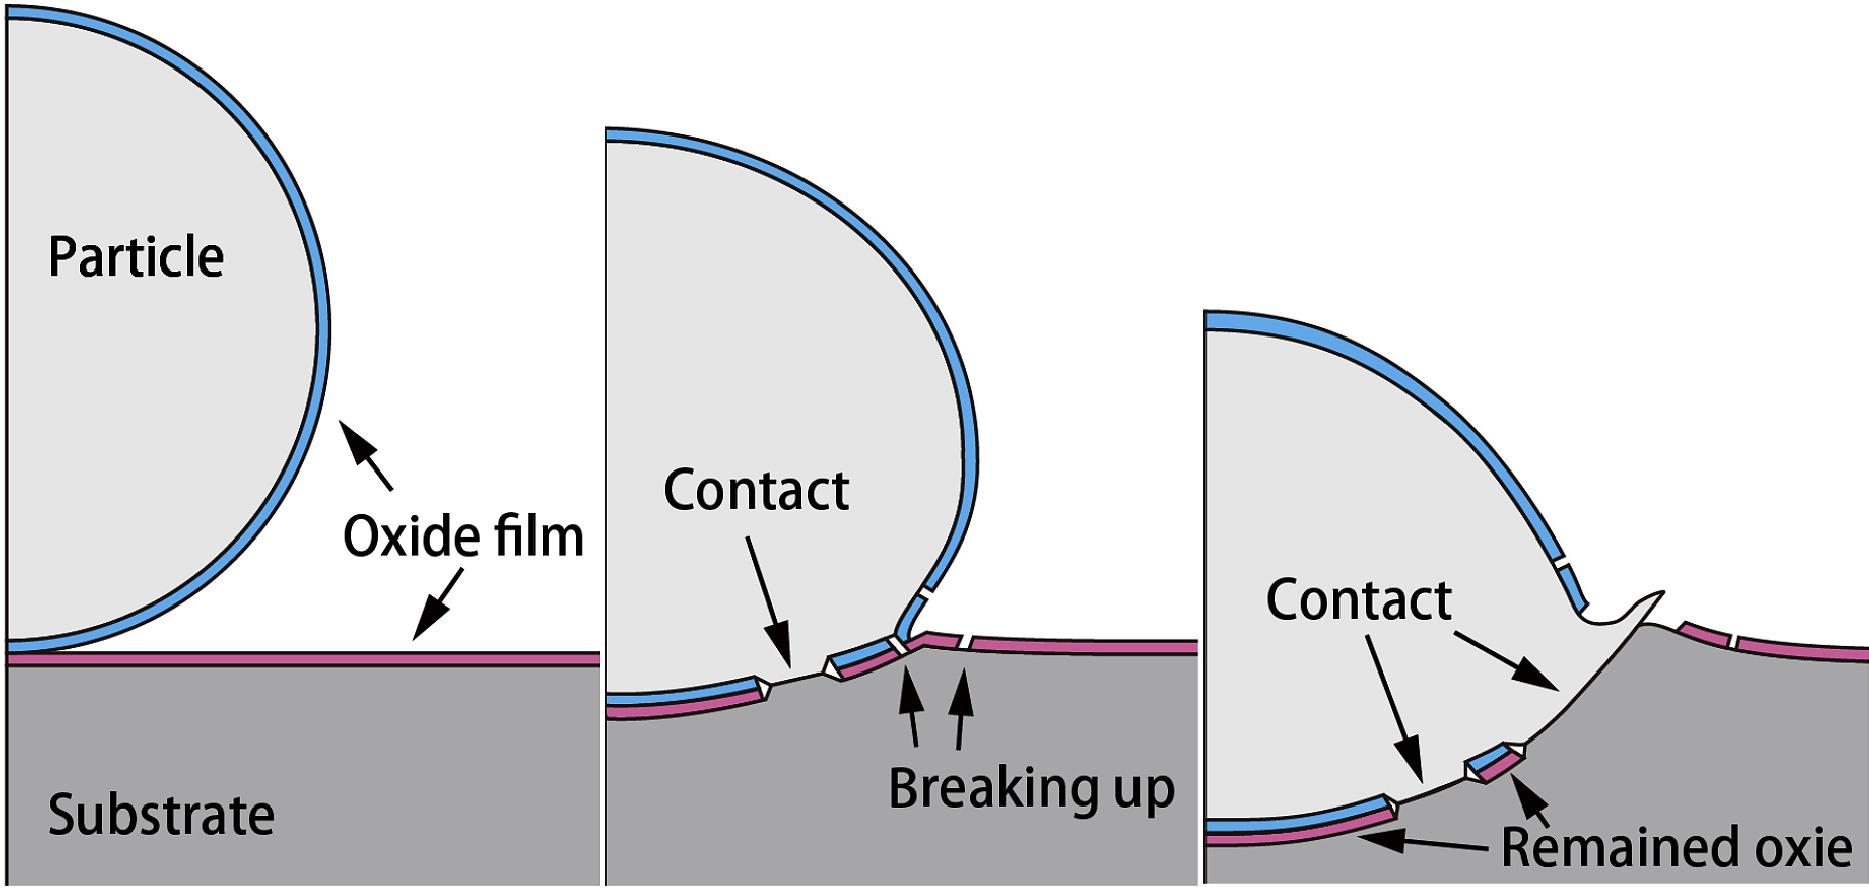
\includegraphics[width=\textwidth]{../report_assets/cs_bonding.png}
        \caption*{Deformation and Bonding on Impact~\cite{ZHANG2024137157}.}
    \end{minipage}
    \hfill
    \begin{minipage}{0.45\textwidth}
        \centering
        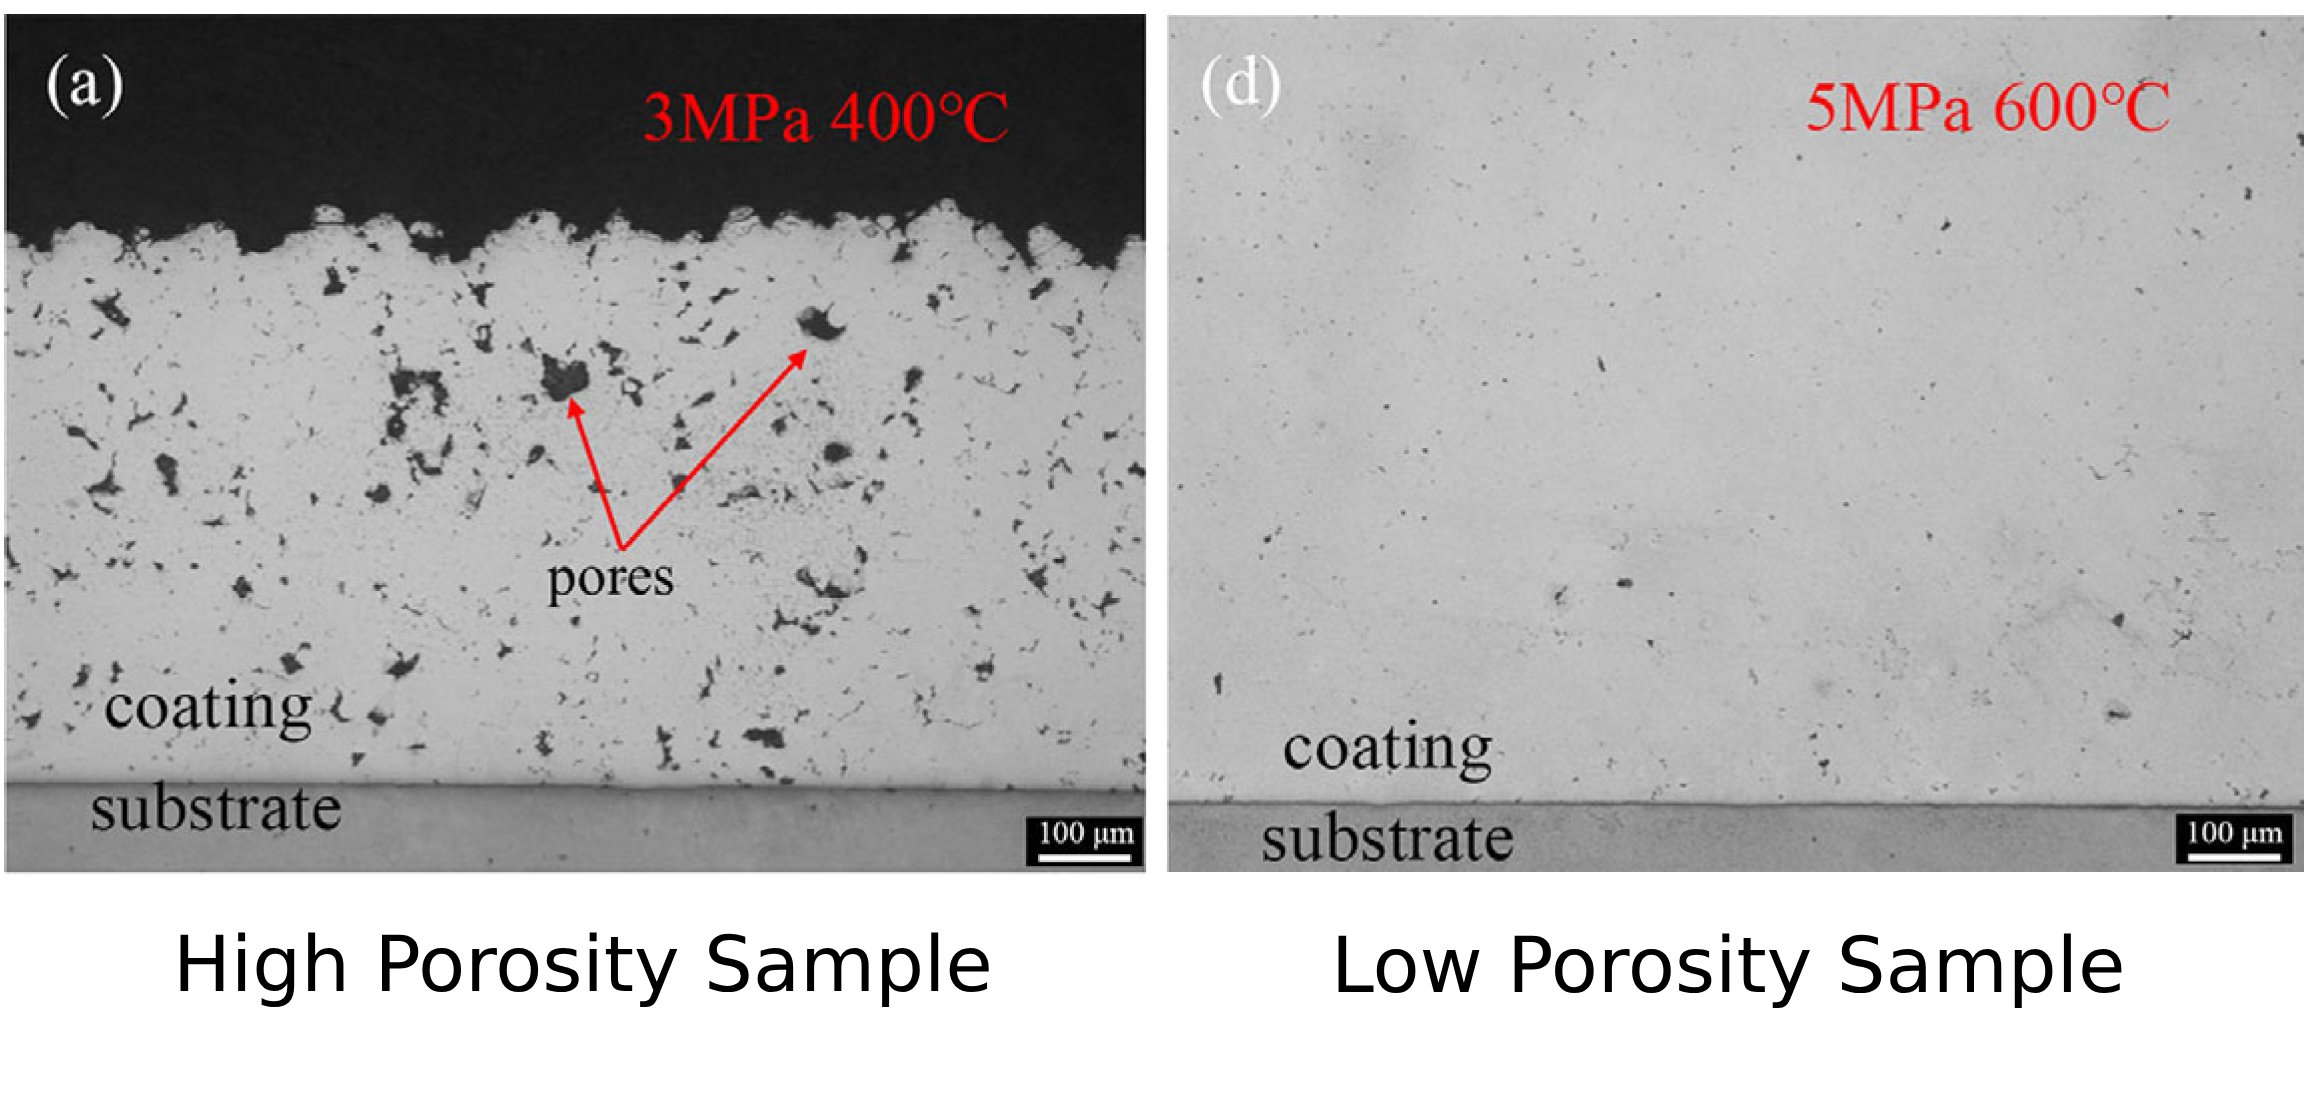
\includegraphics[width=\textwidth]{../report_assets/cs_porosity.png}
        \caption*{Do i need this one?~\cite{coatings13040738}.}
    \end{minipage}
    
\end{figure}\label{fig:fluidisation}
 At this threshold, the pressure drop across the bed reaches a plateau, approximately matching the weight of the solid particles per unit area, and the powder itself begins to swell in volume. The expansion corresponds to an increase in average porosity as particles are pushed further apart in the fluid-like suspension. With further increases in gas flow, the fluidised bed exhibits bubbling behavior. In gas-fluidised systems at ambient pressure, any gas in excess of that needed to just fluidise the bed passes through in the form of buoyant gas voids or bubbles~\cite{SHENG2022137168}.

At the particle scale, motion results from the interplay of buoyancy, drag, and gravitational forces. This is an equilibrium that breaks down in microgravity, making space-based applications particularly challenging to predict or analyse. While the author is aware that research around the topic of particle dynamics under microgravity conditions exists, no research on the behaviour of fluidised powder beds or how to model this in a low gravity regime was found. Therefore, the effects of microgravity on the fluidisation physics has been deemed out of the scope of the project and disregarded.

% \section{Powder Feed Systems}
% Because feedrate of the powder is so influential on the particle velocity and therefore the cold spray process, 
% Powder-feed systems fall into two main paradigms, mechanical and pneumatic, based on the delivery requirements and the properties of the powder they are feeding. Mechanical feeders include rotary-screw units, where powder is metered by the helix speed; vibratory or hopper systems, which use controlled agitation to prevent bridging; and roller or disc designs that finely adjust the gap between rotating elements for high-precision flow. Pneumatic systems split into dense- and dilute-phase conveying: dense-phase moves powder in discrete slugs at low velocity—ideal for fragile or shear-sensitive particles—while dilute-phase entrains powder in a fast airstream for long-distance transfer, at the cost of higher attrition. 

% These feeders underpin key applications like additive manufacturing, thermal spray coatings, powder metallurgy, and pharmaceuticals and food production. 

% Recently, interest around metallic powder fuelled aircraft engines has slowly increased and with it comes the same kind of requirements of a powder feed system as used in in-space manufacturing.

% talk more about this
1-s2.0-S0094576517306124-main look at this for powder particle size impacts
\newpage
\section{Fluidised Powder Feed System Design Evolution}\label{sec:fluidised-powder-feed-systems}
The architecture chosen in \autoref{sec:system_architecture} builds off previous analysis of metallic powder fed engines. A commonly cited first implementation of this pneumatic powder feed system consists of a cylindrical tank with a piston to constrain the powder to the outlet~\cite{LI2021712}. Close to the outlet there is a porous section in which the fluidising gas is supplied. Despite the number of papers referencing this research, the author is unable to validate whether this is still in the public domain. This design was improved upon by pneumatically actuating the piston and supplying the fluidising gas through the piston shaft, with the gas exiting a porous plate mounted on the piston face~\cite{Loftus1972}. 

INVESTIGATE THE SIZE OF THE SETUPS AND FIND PAPER PROVIND WHERE THE REGION OF FLUIDISATION ACTUALLY IS

1-s2.0-S0094576521004446-main for another recap

% Powder feeding in a powder engine under different gas-solid ratios

% The representative and typical fluidised bed powder supply method for powder rocket was proposed by Fricke in powder rocket feasibility evaluation [10]. By referring this idea, the complex fluidised bed powder supply system was improved into Positive Displacement Fluidised Bed (PDFB) supply system by Foote [15]. Meyer improved [16] fluidised bed type powder supply system for the aluminum/magnesium powder rocket, a linear displacement sensor was installed in the piston of the powder supply system to measure the velocity of the piston and calculate the mass flow rate of the powder. Subsequently, Miller [17] added a supplementary air channel at the outlet of the powder storage tank to balance the pressure in the storage tank and improve the stability of the powder feeding system for long time operation. In addition, during the investigation of combustion of dispersions of metal powders, the smaller size powder feeding devices were used to provide micro powder flow rates. Malinin [18] proposed a micro powder feeding device in the investigation of combustion of aluminum-air suspensions, the device consists of a piston with a gas-permeable valve, and a locking and regulating valve with a drive. Similarly, during the study of combustion of boron particles cloud, Yagodnikov [19] optimized the piston, which has a hole through which the transporting gas is passed. Tizilov [20] also used fluidised bed method in his study on flame propagation in aluminum-air mixture flow.

NEED TO FIND PAPER CORRELATING MASS FLOW TO PISTON force
\newpage
\section{Propellent Management Devices}
The need to store material in space is not new and has recieved extensive research, especially regarding the storage of propellants. Like the system presented later, propulsion systems can be disturbed or damaged due to the propellant not being constrained to the outlet~\cite{Hartwig2016}. Common solutions to this problem already exist in the form of propellant management devices.  
\begin{figure}[htbp]
    \centering
    
    \begin{minipage}{0.45\textwidth}
        \centering
        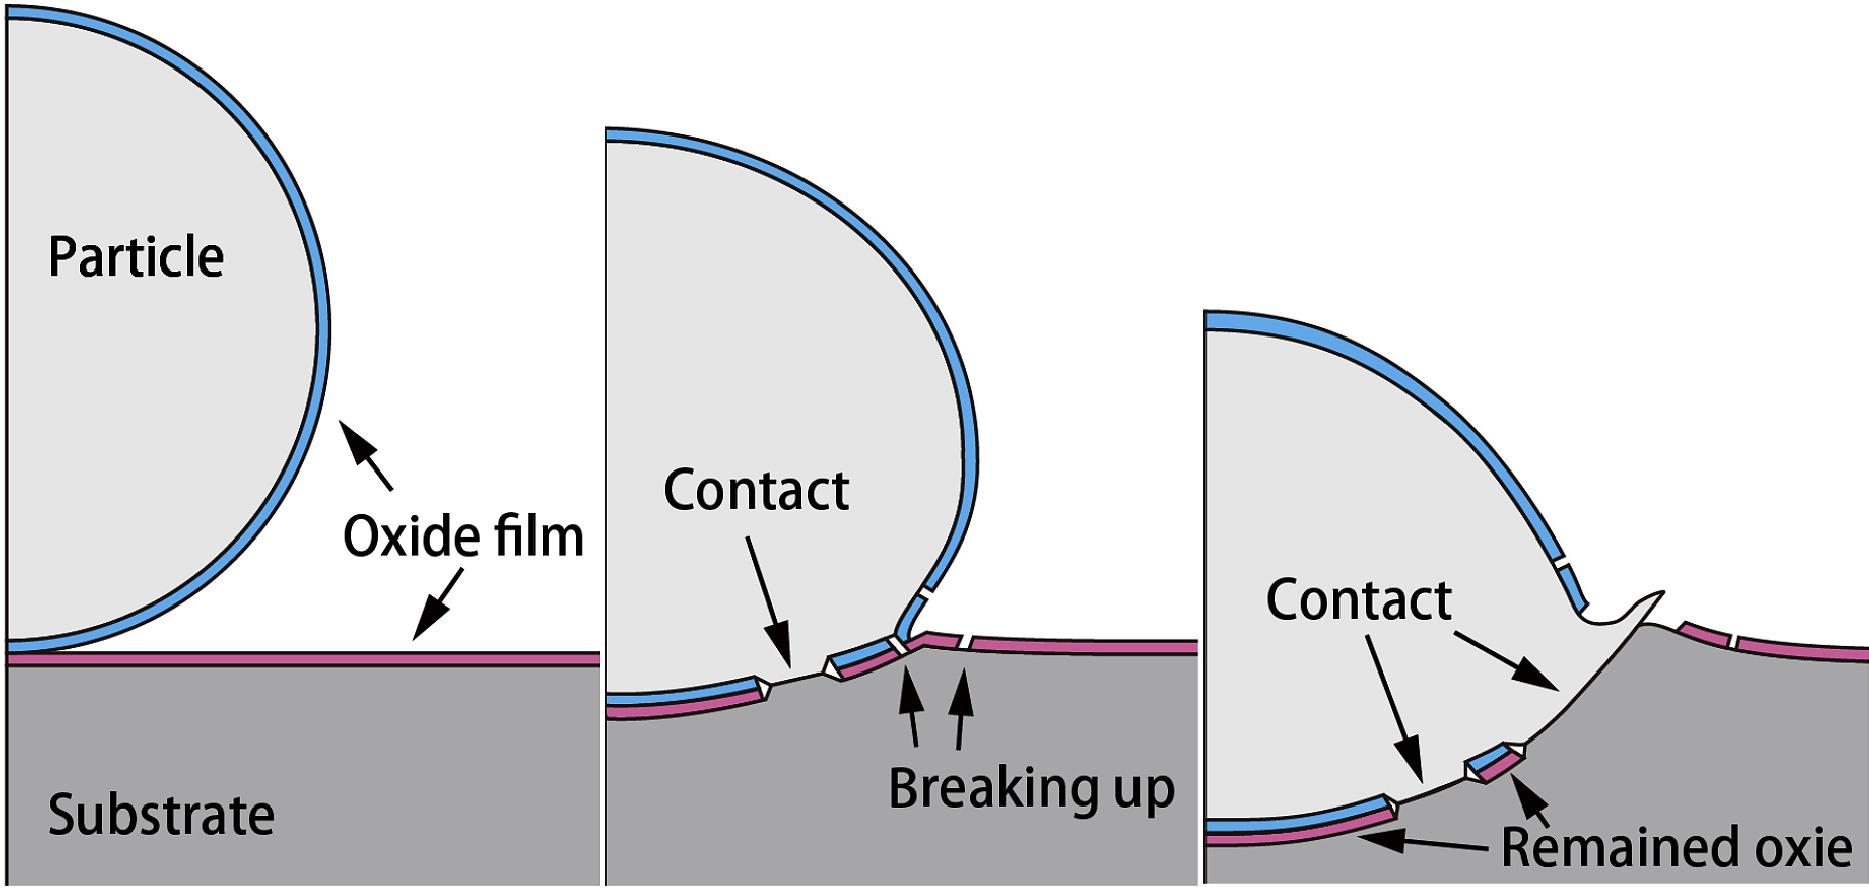
\includegraphics[width=\textwidth]{../report_assets/cs_bonding.png}
        \caption*{Deformation and Bonding on Impact~\cite{ZHANG2024137157}.}
    \end{minipage}
    \hfill
    \begin{minipage}{0.45\textwidth}
        \centering
        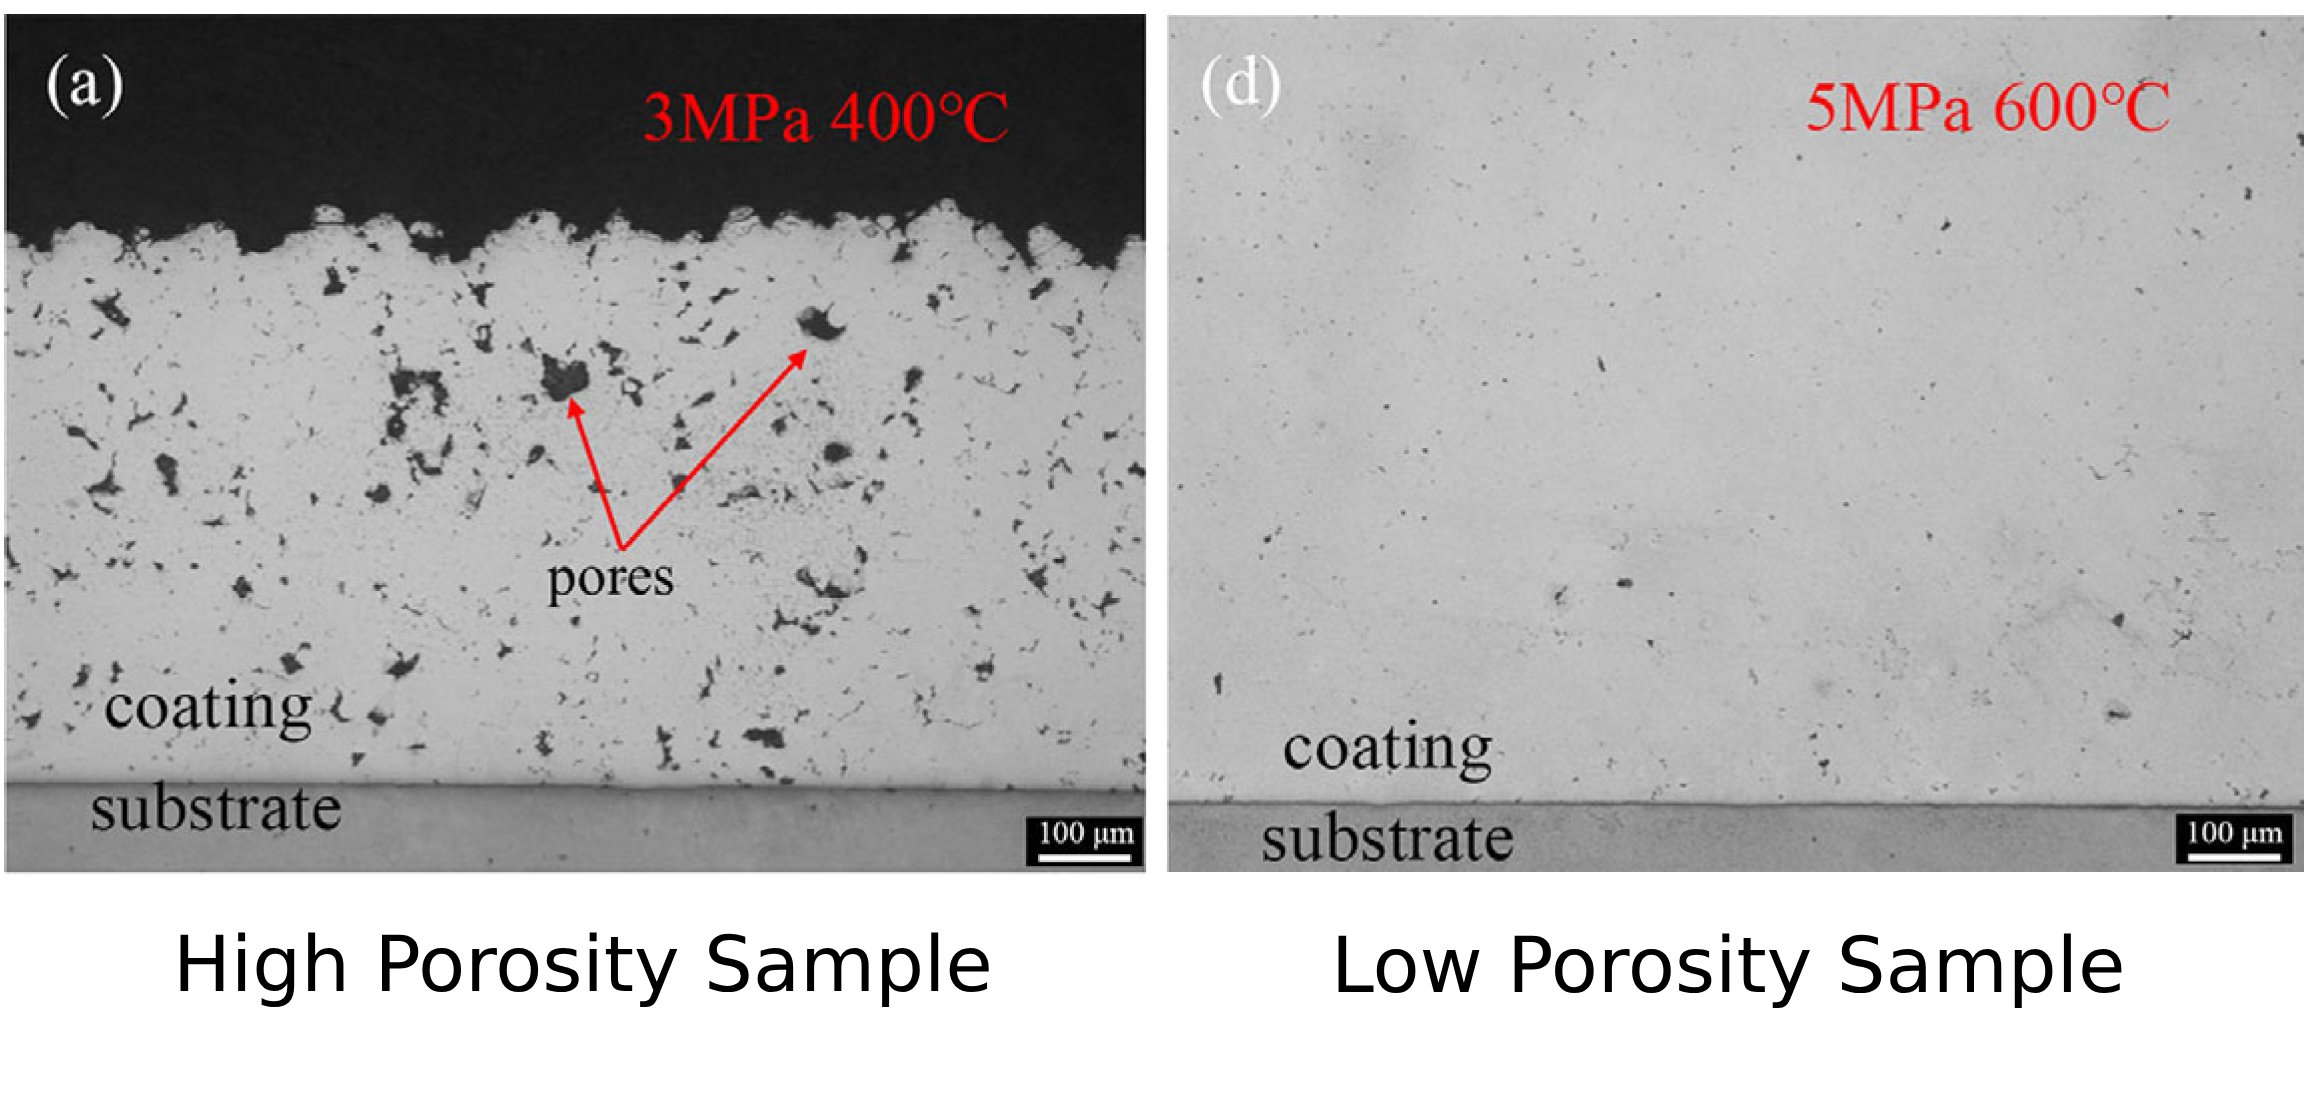
\includegraphics[width=\textwidth]{../report_assets/cs_porosity.png}
        \caption*{Do i need this one?~\cite{coatings13040738}.}
    \end{minipage}
    
\end{figure}\label{fig:pmd}
sloshing phenomenon, surface tension doesnt work, piston tanks and common issues.
1
A Detailed Historical Review of Propellant Management
Devices for Low Gravity Propellant Acquisition
in jan folder
\section{Management of Bulk Powder Phenomenon}
Given that that the storage and distribution of powder is the goal, this section outlines behaviours seen in other systems. A common method of powder storage
\newpage
\section{Modelling Two-phase flow}
There are many different kinds of two-phase flow, from the flow of two immiscible liquids to the solid-gas interactions of interest in this report. Further specifications can be made from the solid-gas category and can be further divided into 3 subcategories: seperated, mixed or transitional and dispersed flow. This analysis is looking at solid particles in a gas and would therefore fall under dispered flows~\cite{enwald1996eulerian}. Enwald, Periano and Almstedt define the general idea as first formulating the integral balance of mass, momentum and energy for the two phases in a fixed control volume. These equations must be satisfied at all points in space and time and therefore can be reduced to two equations, the first concerned with the local instantaneous equations for each phase and the other concerned with the local instantaneous jump conditions. ``IE THE INTERACTIONS BETWEEN PHASES AT THE INTERFACE''??

In principle, this set of equations could be solved by direct numerical simulation but this would require unrealistic computational times. Therefore there are alternative methods like applying a lagrangian approach for the particulate phase but this requires many many equations for the case with many particles and therefore doesnt scale.

Then, the most appropriate method for the case with many particles is the eulerian approach. This works by averaging the local instantaneous equations in either space, time or as an ensemble. The approach relaxes the small mesh and timestep requirements but introduces more unknowns than current equations so requires closure expressions.

The closure laws are of three types: topological, constitutive and transfer laws, where the first type describes the spatial distribution of phase-specific quantities, the second type describes physical properties of the phases and the third type describes different interactions between the phases.~``coppied from source so needs revision''

\subsection{Closing the set of equations}
drag model is a big one, syamal-o'brien has been used so far.gidaspow is better apparently according to this research paper Experimental study and transient CFD/DEM
simulation in a fluidised bed based on different
drag models
will try it and use this as a reason as to why i chose it over others

all models in the paper repeatedly underpredict the bed expansion
\subsection{the chinese research group work}

In addition to the first principles approach, analytical expressions [cite] for the mass flow rate of powder in a fluidised system have been developed and split the regime into a choked system and an unchoked system. The formula for the choked regime, shown in \autoref{equ:1} is simpler, therefore easier to control, and so was used to drive the design choices.

% \begin{align}
%     M &= \frac{P_0 A}{\sqrt{R_m T_0}} \sqrt{\gamma_m} {\left( \frac{2}{\gamma_m + 1} \right)}^{\frac{\gamma_m + 1}{2(\gamma_m - 1)}} \\[10pt]
%     \gamma_m &= \gamma_g \left( 1 + \frac{\phi}{1 - \phi} \frac{C_P}{C_{P,g}} \right) {\left( 1 + \frac{\phi}{1 - \phi} \frac{C_P}{C_{P,g}} \gamma_g \right)}^{-1} \\[10pt]
%     R_m &= \frac{1 - \phi}{1 - \varepsilon} R_g
% \end{align}\label{equ:1}
    
